\documentclass{llncs}

\usepackage{booktabs}
\usepackage{footmisc}
\usepackage{amsmath}
\usepackage{url}
\usepackage{makeidx}
\usepackage{multirow}
\usepackage{graphicx}
\usepackage{float}
\usepackage{titling}
\usepackage{array}
\usepackage{filecontents}
\usepackage{varwidth}
\usepackage{enumitem}


\usepackage{subcaption}
\captionsetup{compatibility=false}

% Footnotes is table
\usepackage{footnote}
\makesavenoteenv{tabular}
\makesavenoteenv{table}

% define dimensions
\setlength{\pdfpageheight}{\paperheight}
\setlength{\pdfpagewidth}{\paperwidth}

% % configure minted
% \usepackage{minted}
% \setminted[bash]{linenos}

% constants
\def\fuzzer{StringFuzz}
\def\generator{\texttt{stringfuzzg}}
\def\transformer{\texttt{stringfuzzx}}

\def\smtfull{SMT-LIB 2.0/2.5}
\def\smt{SMT-LIB}
\def\unix{UNIX}

\DeclareMathOperator{\eval}{eval}

\def\theSuites{\textit{Concats-Balanced}, \textit{Concats-Big},
  \textit{Concats-Extracts-Small}, and \textit{Different-Prefix}}
\def\numSuites{four}

\def\cvc{CVC4}
\def\us{Z3str3}
\def\usOld{Z3str2}
\def\norn{Norn}
\def\theSolvers{\us{}, \cvc{}, \usOld{}, and \norn{}}
\def\numSolvers{four}

\def\linesPerX{45}
\def\linesInFuzzer{3,183}

% \def\problemRepo{\url{https://example.com}}
% \def\sourceRepo{\url{https://github.com/dblotsky/stringfuzz}}

\begin{document}

    % styles
    \pagestyle{headings} % switches on printing of running heads
    \addtocmark{Hamiltonian Mechanics} % additional mark in the TOC

    % title
    \title{
        \fuzzer{}: A Fuzzer for String Solvers
    }
    \titlerunning{\fuzzer{}} % abbreviated title (for running head)

%    % authors
%    \author{
%        Dmitry Blotsky\inst{1}\orcidID{0},
%        Federico Mora\inst{2}\orcidID{0},
%        Murphy Berzish\inst{1}\orcidID{0},\and
%        Yunhui Zheng\inst{3}\orcidID{0},
%        Ifaz Kabir\inst{1}\orcidID{0},
%        Vijay~Ganesh\inst{1}\orcidID{0}
%    }
%    \authorrunning{Dmitry Blotsky et al.}

%    % institutions
%    \institute{
%        University of Waterloo, Waterloo ON, Canada,\\
%        \email{dblotsky@uwaterloo.ca}
%        % U of T for Federico
%        % IBM for Yunhui
%    }

    \maketitle

    \begin{abstract}

    In this paper we present StringFuzz: an SMT-LIB problem fuzzer and generator for string solvers. With it we analyse \numSolvers{} mature string solvers: \theSolvers{}. We use it to craft inputs that elicit poor performance in Z3str3 and CVC4, and provide analyses of the causes of the performance degradations. Our experimental data suggest that there are classes of problems that will always be hard for Z3str3 and easy for CVC4, and vice versa, due to the limitations of the core algorithms implemented by those solvers. We also present several minor bugs in Z3str3 that were exposed by StringFuzz. Finally, we provide a rich repository of problems in SMT-LIB format, generated both by StringFuzz and by hand, to encourage other solver authors to likewise improve their solvers.

\end{abstract}

    \section{Introduction}

In recent years, many algorithms for solving string constraints have
been developed and implemented in SMT solvers such as Norn~\cite{norn},
CVC4~\cite{cvc4}, and Z3 (e.g., Z3str2~\cite{z3str2} and Z3str3~\cite{z3str3}).
To validate and benchmark these solvers, their developers have relied on
hand-crafted input suites~\cite{cvc4-tests,z3str3-tests,z3str2-tests} or
real-world examples from a limited set of industrial
applications~\cite{kaluza,kausler}. These test suites have helped
developers identify implementation defects and develop more
sophisticated solving heuristics. Unfortunately, as solvers grow,
these benchmarks remain stagnant, leaving increasing functionality untested.
As such, there is an acute need for a more robust, inexpensive, and automatic way
of generating benchmarks to test
the correctness and performance of SMT solvers.

Fuzzing has been used to test all kinds of software
including SAT solvers~\cite{fuzzsat}. Inspired by the utility of fuzzers,
we introduce \fuzzer{} and describe its value
as an exploratory testing tool. We demonstrate its efficacy
by presenting limitations it helped discover in
leading string solvers. To the best of our knowledge, \fuzzer{} is the
only tool aimed at automatic generation of string constraints. \fuzzer{} can
be used to mutate or transform existing benchmarks, as well as
randomly generate structured instances. These instances can be scaled with
respect to a variety of parameters, e.g., length of string constants,
depth of concatenations (concats) and regular expressions (regexes),
number of variables, number of length constraints, and many more.

\subsubsection{Contributions}

\begin{enumerate}
    \item \textbf{The \fuzzer{} tool}:
        In Sect.~\ref{sec:fuzzer}, we describe a modular fuzzer that can
        transform and generate \smtfull{} string and regex
        instances.\footnote{We assume basic
        familiarity with string solvers and their input
        language.} Scaling inputs (e.g., long string constants,
        deep concatenations) are particularly useful in identifying asymptotic
        behaviors in solvers, and \fuzzer{} has many options to generate them.
        We briefly document \fuzzer{}'s components and modular architecture.
        We provide example use cases to demonstrate its utility as an
        exploratory solver testing tool.

    \item \textbf{A repository of \smtfull{} instances}:
        We present a repository of \smtfull{} string and regex instance suites
        that we generated using \fuzzer{} in Sect.~\ref{sec:suites}. This
        repository consists of two categories: one with new
        instances generated by \fuzzer{} (\texttt{generated}); and another with
        transformed instances generated from a small suite of industrial
        benchmarks (\texttt{transformed}).

    \item \textbf{Experimental Results and Analysis}:
        We compare the performance of \theSolvers{} on the
        \fuzzer{} suites \theSuites{} in Sect.~\ref{sec:data}. We
        highlight these suites because they make some solvers perform poorly,
        but not others. We analyze our
        experimental results, and pinpoint algorithmic limitations
        in \us{} that cause poor performance.
\end{enumerate}

    \section{\fuzzer{}}
\label{sec:fuzzer}

\subsubsection{Implementation and Architecture}

\fuzzer{} is implemented as a Python package, and comes with several
executables to generate, transform, and analyze \smtfull{} string and regex
instances. Its components are implemented as \unix{} ``filters'' to enable easy
integration with other tools (including themselves). For example, the
outputs of generators can be piped into transformers, and transformers
can be chained to produce a stream of tuned inputs to a
solver. \fuzzer{} is composed of the following tools:
\begin{description}
    \item[\generator{}] \hfill \\
    This tool generates \smt{} instances. It supports several generators and
    options that specify its output. Details can be found in
    Table~\ref{tbl:generators}.
    \item[\transformer{}] \hfill \\
    This tool transforms \smt{}
    instances. It supports several transformers and options that specify
    its output and input, which are explained in
    Table~\ref{tbl:transformers}. Note that transformers
    \textit{Translate} and \textit{Reverse} also preserve
    satisfiability under certain conditions~\cite{ifaz}.
    \item[\texttt{stringstats}] \hfill \\
    This tool takes an \smt{}
    instance as input and outputs its properties: the number of
    variables/literals, the max/median syntactic depth of expressions, the
    max/median literal length, etc.
\end{description}
We organized \fuzzer{} to be easily extended. As evidence of our success we note
that while the whole project
contains \linesInFuzzer{} lines of code, it takes an average of
\linesPerX{} lines of code to create a transformer. \fuzzer{} can either be
installed from source, or from the Python PIP package
repository.\footnote{The link to the source code will be added after double-blind review.}

\begin{table}[t]
    \caption{\fuzzer{} built-in (a) generators and (b) transformers.}
    \begin{subtable}{1\textwidth}
        \centering
        \caption{\generator{} built-in generators.}
        \label{tbl:generators}
        \begin{tabular}{ l l }
            \toprule
            \textbf{Name}
            & \textbf{Generates instances that have ...} \\
            \midrule
            \textit{Concats}
            & Long concats and optional random extracts. \\
            \textit{Lengths}
            & Many variables (and their concats) with length constraints. \\
            \textit{Overlaps}
            & An expression of the form A.X = X.B. \\
            \textit{Equality}
            & An equality among concats, each with variables or constants. \\
            \textit{Regex}
            & Regexes of varying complexity. \\
            \textit{Random-Text}
            & Random, likely syntactically \textit{in}valid text. \\
            \textit{Random-AST}
            & Random, but semantically \textit{valid} text. \\
            \bottomrule
        \end{tabular}
    \end{subtable}
    \begin{subtable}{1\textwidth}
        \centering
        \caption{\transformer{} built-in transformers.}
        \label{tbl:transformers}
        \begin{tabular}{l l}
            \toprule
            \textbf{Name}
            & \textbf{The transformer ...} \\
            \midrule
            \textit{Fuzz}
            & Replaces literals and operators with similar ones.\\
            \textit{Graft}
            & Randomly swaps non-leaf nodes with leaf nodes.\\
            \textit{Multiply}\footnote{Satisfiable inputs
            will produce satisfiable outputs (see Appendix for proof).}
            & Multiplies integers and repeats strings by N.\\
            \textit{Nop}
            & Does nothing (can translate between \smtfull{}).\\
            \textit{Reverse}\footnote{Input and output
            instances will be equisatisfiable (see Appendix for proof).}
            & Reverses all string literals and concat arguments.\\
            \textit{Rotate}
            & Rotates compatible nodes in syntax tree.\\
            \textit{Translate}\footnotemark[4]
            & Permutes the alphabet.\\
            \textit{Unprintable}
            & Replaces characters in literals with unprintable ones.\\
            \bottomrule
        \end{tabular}
    \end{subtable}
\end{table}

\subsubsection{Regex Generating Capabilities}
\fuzzer{} can generate
and transform instances with regular expression constraints. For example, 
\texttt{stringfuzzg regex} invokes the regex
generator and produces an instance of the form:
\begin{align*}
    & \texttt{(assert (str.in.re X}\; R_0\; \texttt{))} \\
    & \texttt{(assert (str.in.re X}\; R_n\; \texttt{))}* \\
    & \texttt{(assert (<= Min (str.len X)))}? \\
    & \texttt{(assert (<= (str.len X)) Max)}?
\end{align*}

where $R_i \in RegEx$, and $Min, Max \in Int$. More simply, the
instance is a set of one or more regex constraints on a single
variable, with optional maximum and minimum length constraints. The
regex constraints $R$ are each of the form:
\begin{align*}
    & \texttt{(re.++}\; T_0\; \texttt{(re.++}\; T_1\;
    \texttt{...}\; \texttt{(re.++}\; T_{n-1}\; T_n\; \texttt{))}
\end{align*}

and each $T_i$ is a recursive term of the form:
\begin{align*}
    & \texttt{(re.*}\; T_{i_j}\; \texttt{) | (re.+}\; T_{i_j}\;
    \texttt{) | (re.union}\; T_{i_{j_1}}\; T_{i_{j_2}}\; \texttt{)}
\end{align*}

where $j$ is the specified depth of recursion. Terms at depth 0 are
regex constants. Informally, this form describes a concatenation of
regex terms, where each term is a random nested regex operator (chosen from
regex Kleene star, repetition, and union), up to a specified depth,
terminating in a regex literal. Below are three example regex instances
(separated by spaces) of depth 2 produced by this scheme:
\begin{align*}
    & ((\texttt{a}|\texttt{b})|(\texttt{cc})+)\quad\quad
    ((\texttt{ddd})*)+\quad\quad ((\texttt{ee})+|(\texttt{fff})*)
\end{align*}

\subsubsection{Equisatisfiable String Transformations}
\fuzzer{} can also transform problem instances.
This is done by manipulating parsed syntax trees.
By default most of the built-in transformers
only guarantee well-formedness, however,
some can even guarantee equisatisfiability. Table~\ref{tbl:transformers}
lists the built-in transformers and notes these guarantees.

\subsubsection{Example Use Case}
In Sect.~\ref{sec:suites} we use \fuzzer{} to generate benchmark suites in a batch mode.
We can also use \fuzzer{} for on-line exploratory debugging.
For example, the script below repeatedly feeds random \fuzzer{}
instances to \cvc{} until the solver produces an error:
{\scriptsize\begin{verbatim}
while stringfuzzg -r random-ast -m \
    | tee instance.smt25 | cvc4 --lang smt2.5 --tlimit=5000 --strings-exp; do
    sleep 0
done\end{verbatim}}

    \section{Instance Suites}
\label{sec:suites}

In this section, we describe the benchmark suites we generated
with \fuzzer{}, and on which we conducted our experimental
evaluation. Table~\ref{tbl:generated} lists instances that were
generated by \generator{}. Table~\ref{tbl:transformed} lists instances
derived from existing seed instances by iteratively applying \transformer{}.
Every transformed instance is named according to its
seed and the transformations it undertook. For example,
\texttt{z3-regex-1-fuzz-graft.smt2} was transformed by applying
\textit{Fuzz} and then \textit{Graft} to \texttt{z3-regex-1.smt2}.

The \textit{Amazon} category contains 472 instances derived from two seeds
supplied by our industrial collaborators. The \textit{Regex} category is
seeded by the \usOld{} regex test suite~\cite{z3str2-tests}, which contains
42 instances. Through cumulative transformations we expanded the
42 seeds to 7,551 unique instances. Finally, the \textit{Sanitizer} category
is obtained from five industrial e-mail address and IPv4 sanitizers.

\begin{table}[t]
    \caption{Repository of 10,258 \smtfull{} instances.}
    \begin{subtable}{1\textwidth}
        \centering
        \caption{\generator{}-generated instances.}
        \label{tbl:generated}
        \begin{tabular}{llr}
            \toprule
            \textbf{Name}
                & \textbf{Instances have a ...}
                & \textbf{Quantity}
            \\
            \midrule
            \textit{Concats-\{Small,Big\}}
                & Right-heavy, deep tree of concats.
                & 120 \\
            \textit{Concats-Balanced}
                & Balanced, deep tree of concats.
                & 100 \\
            \textit{Concats-Extracts-\{Small,Big\}}
                & Single concat tree, with character extractions.
                & 120 \\
            \textit{Lengths-\{Long,Short\}}
                & Single, large length constraint on a variable.
                & 200 \\
            \textit{Lengths-Concats}
                & Tree of fixed-length concats of variables.
                & 100 \\
            \textit{Overlaps-\{Small,Big\}}
                & Formula of the form A.X = X.B.
                & 80 \\
            \textit{Regex-\{Small,Big\}}
                & Complex regex membership test.
                & 120 \\
            \textit{Many-Regexes}
                & Multiple random regex membership tests.
                & 40 \\
            \textit{Regex-Deep}
                & Regex membership test with many nested operators.
                & 45 \\
            \textit{Regex-Pair}
                & Test for membership in one regex, but not another.
                & 40 \\
            \textit{Regex-Lengths}
                & Regex membership test, and a length constraint.
                & 40 \\
            \textit{Different-Prefix}
                & Equality of two deep concats with different prefixes.
                & 60 \\
            \bottomrule
        \end{tabular}
    \end{subtable}

    \begin{subtable}{1\textwidth}
        \centering
        \caption{\transformer{}-generated instances.}
        \label{tbl:transformed}
        \begin{tabular}{llr}
            \toprule
            \textbf{Name}      & \textbf{Seed}                              & \textbf{Quantity} \\
            \midrule
            \textit{Amazon}    & Two industrial regex membership instances. & 472 \\
            \textit{Regex}     & Z3str2 regular expression test suite.      & 7,551 \\
            \textit{Sanitizer} & Five e-mail and IPv4 sanitiser examples.   & 1,170 \\
            \bottomrule
        \end{tabular}
    \end{subtable}
\end{table}

    \section{Experimental Results and Analysis}
\label{sec:data}

We generated several problem suites with \fuzzer{} that made one
solver perform poorly, but not others. These suites are
\theSuites{}. Figure~\ref{fig:cvc-hard} shows the suites that were
uniquely difficult for \cvc{}. Figure~\ref{fig:z3str3-hard} shows the
suites that were uniquely difficult for \us{}. All experiments were
run in series, with a timeout of 15 seconds, on the same computer running
Ubuntu Linux 16.04. The computer had 32GB of RAM and an
Intel\textregistered{} Core\texttrademark{} i7-6700 CPU with clock speed
of 3.40GHz.

\begin{figure}[h]
    \begin{subfigure}{.5\textwidth}
        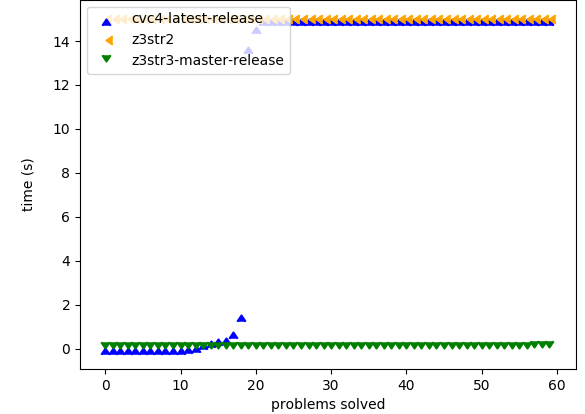
\includegraphics[width=\textwidth]{data/graphs/concats-extracts-small.png}
        \caption{Performance on concats-extracts-small}
        \label{fig:concats-extracts-small}
    \end{subfigure}
    \begin{subfigure}{.5\textwidth}
        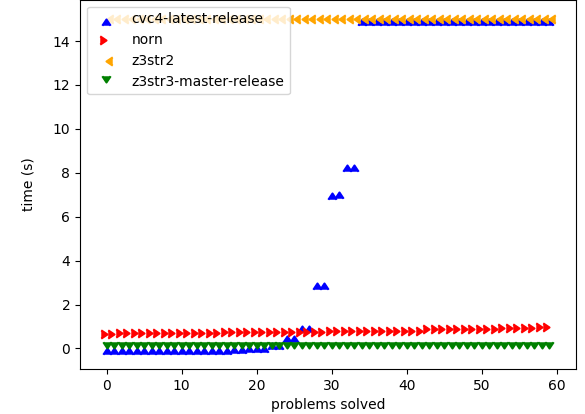
\includegraphics[width=\textwidth]{data/graphs/different-prefix.png}
        \caption{Performance on different-prefix}
        \label{fig:different-prefix}
    \end{subfigure}
    \caption{Problems hard for \cvc{}}
    \label{fig:cvc-hard}

    \begin{subfigure}{.5\textwidth}
        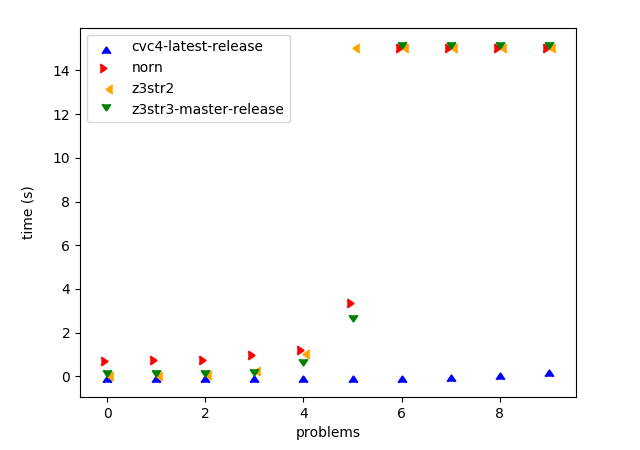
\includegraphics[width=\textwidth]{data/graphs/concats-balanced.png}
        \label{fig:concats-balanced}
        \caption{Performance on concats-balanced}
    \end{subfigure}
    \begin{subfigure}{.5\textwidth}
        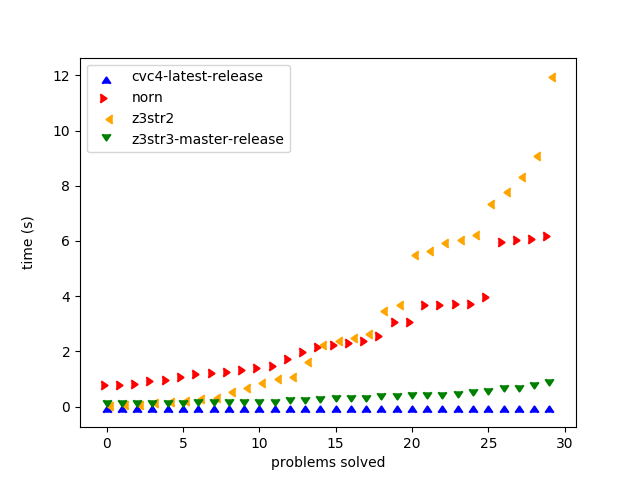
\includegraphics[width=\textwidth]{data/graphs/concats-small.png}
        \label{fig:concats-small}
        \caption{Performance on concats-small}
    \end{subfigure}
    \caption{Problems hard for \us{}}
    \label{fig:z3str3-hard}
\end{figure}

\subsubsection{Usefulness to \us{}: A Case Study}

We found a number of performance-related issues and opportunities for
new heuristics in \us{} thanks to \fuzzer{}. For example, the
instances in the \textit{concats-big} suite generated by \fuzzer{}
helped us discover a missing heuristic. In particular, \us{} didn't
make full use of the solving context (e.g. some terms are empty
strings) to simplify the concatenations of a long list of string terms
before trying to reason about the equivalences among subterms. \us{}
therefore introduced a large number of unnecessary intermediate
variables and propagations. As an immediate consequence of
testing \us{} on \textit{concats-big} benchmarks, we were able to
identify the factors common to these instances and rapidly formulate a
hypothesis as to why they were performing poorly.

    \section{Related Work}

Naturally, many solver developers author their own test suites to
validate their solvers~\cite{cvc4-tests,z3str3-tests,z3str2-tests}. In
addition, several popular problem suites are publicly available for
solver validation, such as the Kaluza~\cite{kaluza} and
Kausler~\cite{kausler} suites. There are likewise several fuzzers and
problem generators currently available, but none of them can generate
or transform string and regex problems. For example, the
FuzzSMT~\cite{fuzzsmt} tool generates \smt{} problems with bit-vectors
and arrays, but does not support strings or regexes. The
SMTpp~\cite{smtpp} tool pre-processes and simplifies problems, but
does not generate new ones or fuzz existing ones.


    \bibliographystyle{abbrv}
    \bibliography{paper}

    \newpage
    \appendix
    \section{Appendix}

In this section, we informally discuss how we established
equisatisfiability guarantees regarding the transformations provide in
\fuzzer{}. We assume that the reader is familiar with SMT-LIB
syntax. The transformations work over boolean, integer, string
literals and expressions, and regular expressions.

To shorten our proofs, we make the following simplifications:
\begin{enumerate}
  \item
    Since many of the operators can be expressed in terms of others,
    our proofs will only consider a subset of the operators. In
    particular we drop the following:
    \begin{itemize}
      \item \texttt{||} (boolean or)
      \item \texttt{=} for boolean expressions
      \item \texttt{<=}, \texttt{>}, \texttt{>=}
      \item \texttt{str.prefixof}, \texttt{str.suffixof}, \texttt{str.at}, \texttt{str.contains}
      \item \texttt{re.range}, \texttt{re.+}, \texttt{re.allchar}, \texttt{re.all}
    \end{itemize}

  \item
    In the above, we assume that \texttt{str.at} is expressible using
    \texttt{substring} although the semantics slightly differ when the index is
    out of bounds.
\end{enumerate}

\begin{definition}
  A \emph{model} is a mapping from boolean, integer, and string variables to
elements in the domain of universe of the corresponding type.
\end{definition}

\begin{definition}
  A \emph{formula} $P$ satisfies a model $m$ if $P$ evaluates to
  \texttt{true} under the model $m$. The function $\eval (P)$
  evaluates a formula under a model; the specific model used is left
  implicit as it is clear from context.
\end{definition}

The proofs all follow a very similar structure. For each
transformation \textit{Trans}, we show that a formula $P$ is
satisfiable by a model $m$ if and only if $\textit{Trans}(P)$ is
satisfiable by $\textit{Trans}(m)$, where $\textit{Trans}(m)$ is the
transformation applied to all the constants in the model $m$. (The
exception here is the \textit{Multiply} operator as discussed below.)

To show the above, we show that for all expressions $e$,
$\textit{Trans}(\eval (e)) = \eval (\textit{Trans}(e))$. This is
proven using a straightforward induction on the structure of
expressions. Since the transformations fix boolean constants, we have,
$\textit{Trans}(\eval (P)) = \eval (P)$, and hence if the original
problem is satisfiable so is the transformed problem.

For transformations that have an inverse, such as \textit{Translate}
and \textit{Reverse} this also shows that if the transformed problem
is satisfiable, then the original problem is satisfiable, proving that
they are equisat transformations. \textit{Multiply} (as defined here)
does not have an inverse and hence it only guarantees to take
satisfiable problems to satisfiable problems. This can be seen in the
problem instance $y<x<y+1$ which is UNSAT, but multiplying by 2
transforms the problem into $y<x<y+2$ which is SAT.

\subsection{Translate}
We now prove that \textit{Translate} transforms constraints into
equisatisfiable constraints. From above, we only need to show that for
every expression $e$, the following is true: $\textit{Translate}(\eval
(e))$ = $\eval (\textit{Translate}(e))$. For now, we assume that
\textit{Translate} fixes the digits pointwise and we prove the
stronger fact that $\textit{Translate}$ also fixes characters
pointwise in any string expression. (I.e., $\textit{Translate}$ are
bijections and further that digits are not mapped to any other
character.)

It is clear that for literals $l$, $\textit{Translate}(\eval (l)) =
\eval (\textit{Translate}(l))$. Then, assuming that the it holds for
smaller expressions, we show that it holds larger expressions $e$
created using the constructs \texttt{and}, \texttt{=} (for strings and
integers), \texttt{+}, \texttt{-}, \texttt{*}, \texttt{str.len},
\texttt{str.indexof}, \texttt{str.++}, and \texttt{str.substr}.

For \texttt{str.in.re} we had to show that a string literals $s$, is a
member of a regular expression $r$ if and only if
$\textit{Translate}(s)$ is a member of $\textit{Translate}{r}$ by
induction on regular expressions. For the inductive cases of
\texttt{str.to.int}, and \texttt{str.from.int} we needed to use the
fact that the digits were fixed pointwise.

The restriction that \textit{Translate} must fix the digit characters
can be relaxed if we are translating problem instances that do not use
\texttt{str.to.int} or \texttt{str.from.int}. Without these operators
we can show $\textit{Translate}(\eval (e))$ = $\eval
(\textit{Translate}(e))$ directly by induction without having to worry
about fixing digits pointwise.

\subsection{Reverse}
\textit{Reverse} does not transform constraints that use
\texttt{str.replace}, \texttt{str.indexof}, \texttt{str.to.int}, and
\texttt{str.from.int}. These operators do not have a well-defined
notion of a reverse. The required lemma is proved by induction on the
rest of the operators similar to proof for \textit{Translate}.

We end our discussion on \textit{Reverse} by noting that although it
disallowed \texttt{str.replace}, it only did so because it didn't have
a natural notion of a reverse in the theory we were working with.
%% If we expand our theory to also include an operator that replaces
%% the last instance, we can transform problems that use
%% \texttt{str.replace}.

\subsection{Multiply}
\textit{Multiply} does not transform constraints that use \texttt{*},
\texttt{str.indexof}, \texttt{str.to.int}, and
\texttt{str.from.int}. These operators do not have a well-defined
notion of a multiply. The required lemma is proved by induction on the
rest of the operators similar to the above proofs.

We disallow \texttt{*} for \textit{Multiply} because of problems
instances such as \texttt{(= 10 (* 2 5))}. A naive \textit{Multiply}
by $3$ would transform this satisfiable problem into the unsatisfiable
\texttt{(= 30 (* 6 15))}.


    % \appendix
    % \section{Appendix}

\end{document}
